\chapter{Results and interpretation}\label{chap:results}
\minitoc
Now that all backgrounds are well estimated, the background prediction is reliable in the validation region, and all uncertainties are determined, the background prediction methods can be applied to the SR, $\ptmiss>150\GeV$ and $\mtTwo>100\GeV$, and predicted and observed event counts can be compared. An excess of events or other significant deviations from the prediction could be indicators for BSM physics.
\section{Results}\label{sec:results}
\subsection*{Signal region binning}
In order to perform the counting experiment, a distinct binning in one or multiple variables needs to be applied to the SR. This binning can be optimized considering different criteria, \eg, observation and exclusion power. Since the most sensitive variables are $\ptmiss$ and $\mtTwo$, different one dimensional and two dimensional binnings are possible.
% For signal benchmark points of all three signal models, simplified significances $\frac{s}{\sqrt{s+b}}$, where s is the number of signal events and b the number of background events per bin, the binnings are varied.
Because the total predicted event count in the SR is approximately $13$ events, special care has to be taken regarding this low data yield. Albeit many sensitive bins with lower SM prediction and high signal expectation would push expected exclusion limits, this would make reinterpretations and observations difficult due to the high statistical uncertainties of the measured data. Considering that the $\ptmiss$ and $\mtTwo$ distributions are exponentially decreasing for the predicted backgrounds, the maximum number of bins is limited. Therefore, a binning consisting of two bins is chosen. It consists of two bins in the $\ptmiss$ distribution, as already introduced in \refSec{sec:SRSelection}. The first bin starts at $150\GeV$ and ends at $200\GeV$, while the second one gathers all events with $\ptmiss>200\GeV$ in the SR. This choice yields good exclusion power while containing a sufficient number of events in each bin, so that the reinterpretation is not restricted by statistical uncertainties. For the same reasons, higher dimensional binnings are discarded, too. The $\ptmiss$ distribution is preferred over the $\mtTwo$ distribution, because it is more model independent given the many decay possibilities in full theoretical models. In the calculation of $\mtTwo$, both bosons are assumed to be generated in an NLSP decay together with a gravitino, but the relevant final state particles ($\PZ$ and $\PGg$) can be produced in several decay branches of different particles considering consistent models. In contrast, $\ptmiss$ is a general measure of the energy carried by the gravitinos, thus being more independent and universal.
% This binning yields good exclusion power, because the $\ptmiss$ distribution is observed to be more sensitive than the $\mtTwo$ distribution, and includes an amount of events large enough in each bin, so that the reinterpretation is not restricted by statistical uncertainties. For the same reasons, higher dimensional binnings are discarded.
\subsubsection*{Possible influence of signal to the validation region}
The SR and the VR are very close to each other in phase space due to the chosen sideband structure of the VR. Thus, some signal events, especially for low SUSY masses, are expected to populate also the VR. The distribution most sensitive to this effect is the $\pt^{\PGg}$ distribution of the selected photon, as shown in \refFig{fig:signalContVR}, where the $\pt^{\PGg}$ and $\ptmiss$ distributions are compared.
\begin{figure}[tbp]
 \centering
 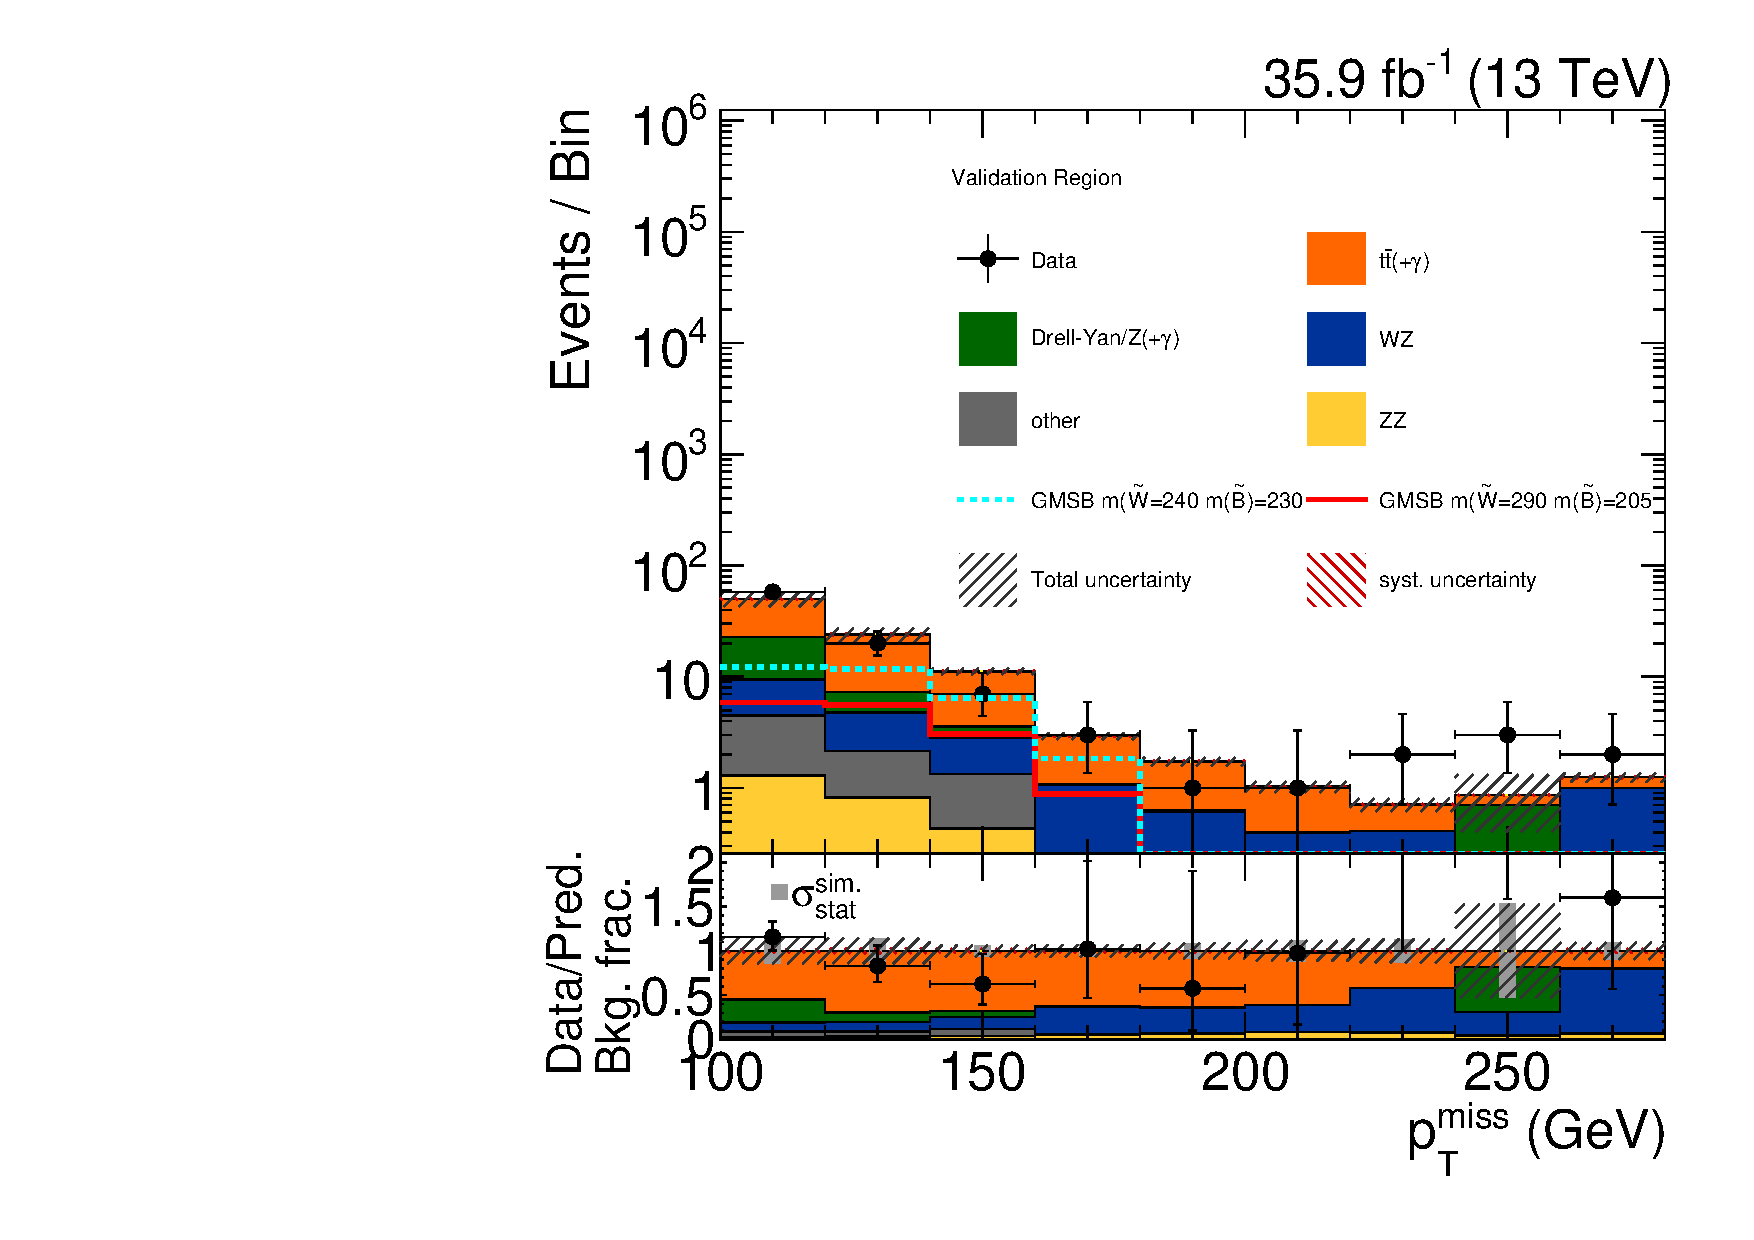
\includegraphics[width=\pairwidth]{figures/VR_signal_study/VR_LL_met_log}
 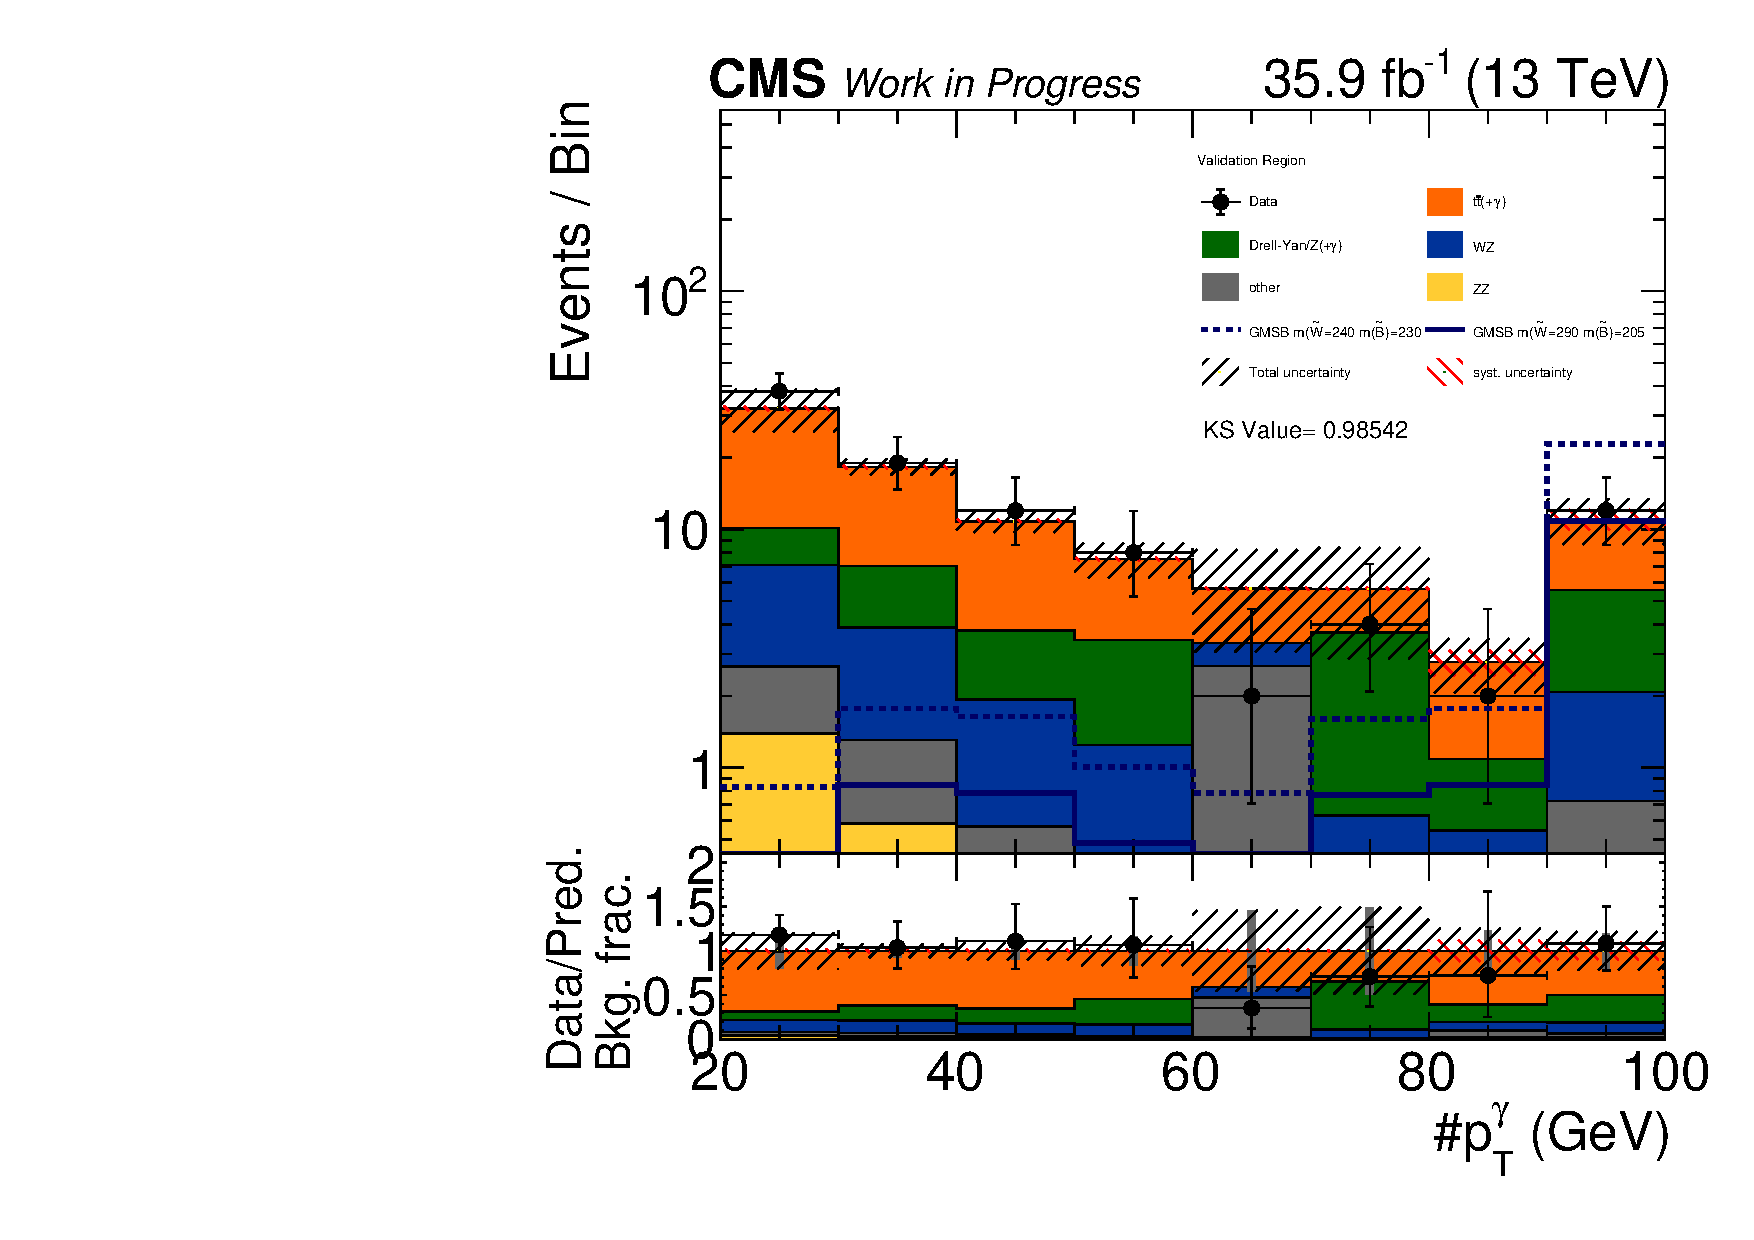
\includegraphics[width=\pairwidth]{figures/VR_signal_study/VR_LL_pt_g1_log}
 \caption{The $\ptmiss$ (left) and transverse momentum distribution of the photon in the VR (right). Signal benchmark points are also added to show the possible sensitivity in the high $\pt^{\PGg}$ regime.}
 \label{fig:signalContVR}
\end{figure}
For $\pt^{\PGg} >80\GeV$, a considerable amount of signal events is measurable in the VR, because in the considered SUSY processes the photons produced in the NLSP decay gain high momenta due to the high NLSP masses. Since the predicted background and observed data are already compared in the VR, and no background prediction is performed here, there is no need to account for this effect like in the other CR in terms of signal contamination.\\
Hence, the subtraction of this region from the VR, and the addition to the SR as a third search bin would increase the total sensitivity. The number of expected signal events in the two SR bins is already high enough for the relevant signal points to be excluded with a high significance. Thus, this strategy does not show any improvement in the overall sensitivity, that is large enough to justify the deterioration in the simplicity of the analysis.


\subsection*{Signal acceptances}
The acceptance of the event selection is defined as the fraction of events being selected in the SR to all events in a distinct SUSY signal scenario being produced before passing the reconstruction, identification, and selection. Because several effects are considered in the definition, such as detector acceptance and trigger efficiencies, it is often referred to as acceptance times efficiency. In \refTab{tab:cutflow}, exemplary the events yields for three different signal points after several analysis steps are given. In addition, the relevance of each SR bin with regard to the final sensitivity is indicated by comparing the expected number of signal events in each bin.\\
For all three considered signal scenarios, the acceptance after the preselection is already of the order of $\mathcal{O}(1\%)$. Due to the low branching fraction of the $\PZ$ boson decaying to either an electron or a muon pair (each approximately $3.36\%$), low acceptances are expected considering the inefficiencies of the reconstruction, the trigger, and the particle identification. In addition, the probability for the NLSP to decay to a Z boson is only $50\%$ in the SMS, and even lower for the GMSB model, see \refSec{sec:SMS}. Therefore, the total acceptance is further decreased. The SR selection requirements, namely the $\ptmiss$ and $\mtTwo$ requirements, reduce the signal yield only insignificantly while decreasing the background contributions. Signal acceptances for all signal points are given in \refSec{sec:app_signal} in the appendix. Comparing the acceptances for all points, they are all of the same order, slightly depending on the sparticle masses.

\begin{table}[h!]
 \centering
 \caption{Number of events for three signal points after several selection steps. The signal points correspond to the \texttt{TChiZG} model with $m(\mathrm{NLSP})=600\GeV$, the GMSB model with $m(\widetilde{W})=415\GeV$ $m(\widetilde{B})=355\GeV$ , and the \texttt{T5bbbbZG} model with $m(\tilde{g})=1500\GeV$ $m(\mathrm{NLSP})=1400\GeV$.}
 \normalsize
 \label{tab:cutflow}
 \begin{tabular}{lllllll}
                            & \multicolumn{6}{c}{Number of Events (Rel. fraction)}                                                                                                      \\\hline
  Selection                 & \multicolumn{2}{c}{\texttt{TChiZG}}                  & \multicolumn{2}{c}{GMSB} & \multicolumn{2}{c}{\texttt{T5bbbbZG}}                                   \\\hline
  Before Selection          & $1063$                                               & ($100\%$)                & $5285$                                & ($100\%$)  & $509$ & ($100\%$)  \\
  Preselection              & $11.3$                                               & ($1.06\% $)              & $21.5$                                & ($0.40\%$) & $5.1$ & ($1.00\%$) \\
  $\mtTwo>100\GeV$          & $10.8$                                               & ($1.02\%$)               & $18.5$                                & ($0.35\%$) & $5.0$ & ($0.99\%$) \\
  $\ptmiss>150\GeV$         & $9.8$                                                & ($0.92\%$)               & $14.2$                                & ($0.27\%$) & $4.9$ & ($0.96\%$) \\\hline
  $150\GeV<\ptmiss<200\GeV$ & $0.7$                                                & ($0.06\%$)               & $3.2$                                 & ($0.06\%$) & $0.1$ & ($0.02\%$) \\
  $\ptmiss>200\GeV$         & $9.1$                                                & ($0.86\%$)               & $11.0$                                & ($0.21\%$) & $4.8$ & ($0.94\%$) 
 \end{tabular}
 \vspace{\baselineskip}
\end{table}


\subsection*{Event yields}
The final background prediction together with the observed event yield is shown in \refFig{fig:result}.
The total background uncertainties are obtained by adding the individual uncertainties quadratically. The statistical uncertainties in the measurement are calculated using $68\%$ confidence intervals of the Poisson distribution with the mean set to the observed yield.
To show the effect of a possible signal in the counting experiment, contributions of two example signal points are drawn for comparison.\\
The number of background and observed events together with their total uncertainties are given also in \refTab{tab:results}. The measured data yields are in good agreement with the predicted background events, thus no evidence for BSM physics is found. The measured excess corresponds to a significance of $1.3$ standard deviations calculated with the discovery significance based on a profile-likelihood ratio test and Asimov approximation~\cite{Significance2}
\begin{equation}
 Z_A = \left[ 2\left( n\ln{\left[\frac{n(b+\sigma_{b}^2)}{b^2+n\sigma_{b}^2}\right]} -\frac{b^2}{\sigma_{b}^2} \ln \left[1+\frac{\sigma_b ^2 (n-b)}{b(b+\sigma_b ^2)} \right]  \right)    \right]^{1/2},
\end{equation}
where $n$ is the observed yield, $b$ the predicted background, and $\sigma_{b}$ the total uncertainty on the prediction, combining the statistical and systematic uncertainty on the background prediction.\\
Albeit other approaches to calculate the observed significance, like $\frac{n-b}{\sqrt{b}}$ and $\frac{n-b}{\sqrt{b+\sigma_b^2}}$, overestimate the significance for small $b$, the Asimov significance yields a more confident estimate of the true significance of the observation~\cite{Significance}.
\begin{figure}[bpt]
 \centering
 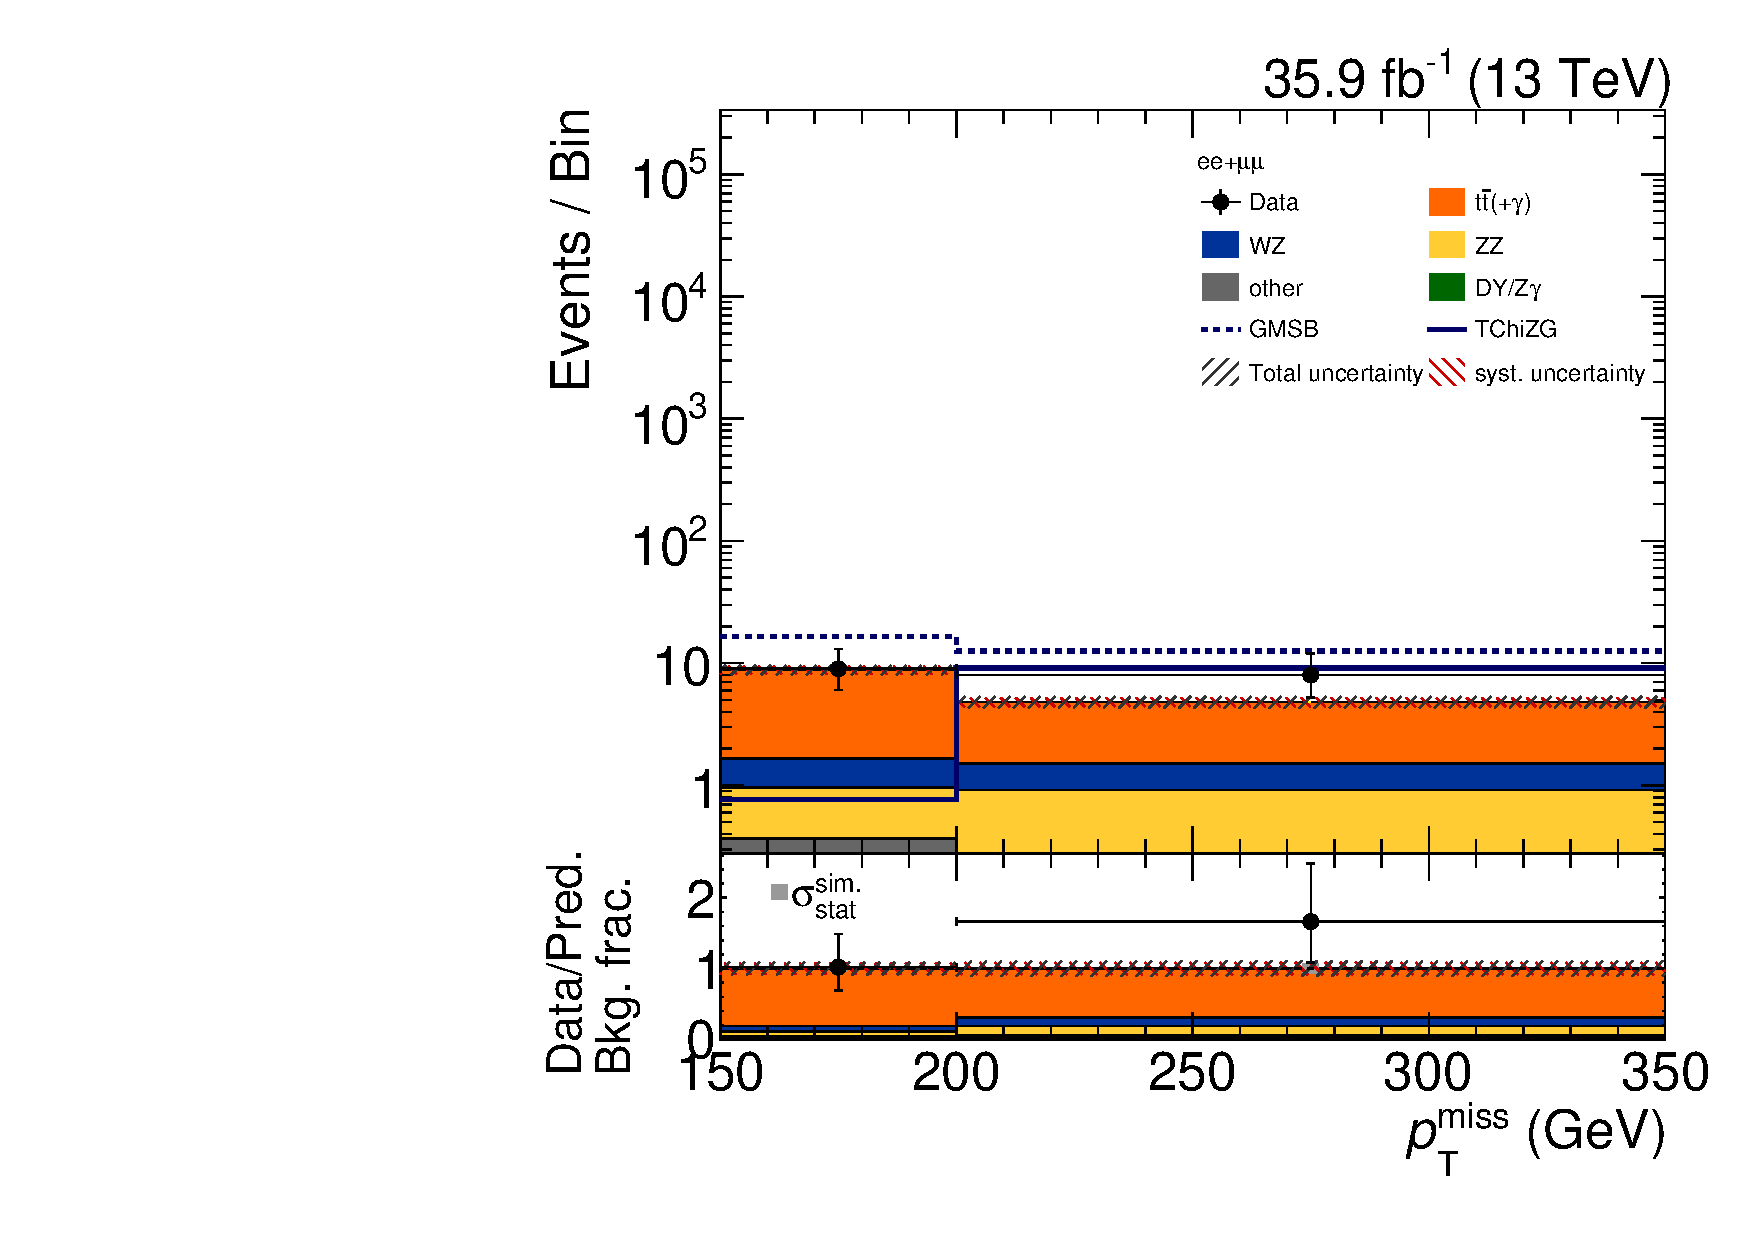
\includegraphics[width=0.7\textwidth]{figures/EndorsementPlots/final_MC_log}
 \caption{Comparison between final prediction and observation with statistical and systematic uncertainties in the signal region. Two signal expectations for the \texttt{TChiZG} model with $m(\text{NLSP})=600\GeV$ and the GMSB model with $m(\tilde{W})=290\GeV$ and $m(\tilde{B})=205\GeV$ are also shown.}
 \label{fig:result}
\end{figure}
\begin{table}[bpt]
 \centering
 \caption{Observed yields and final predicted background yields with the statistical and systematic uncertainties for each bin and background.}
 \normalsize
 \label{tab:results}
 \begin{tabular}{lllllll}
  $\ptmiss$      & \multicolumn{3}{l}{$150-200\GeV$} & \multicolumn{3}{l}{$200\GeV-\infty$}                                                               \\\hline
                 & yield                             & $\sigma_{stat}$                      & $\sigma_{syst}$ & yield & $\sigma_{stat}$ & $\sigma_{syst}$ \\\hline
  $\ttbar(\PGg)$ & 7.16                              & 0.32                                 & 0.60            & 3.31  & 0.23            & 0.37            \\
  DY/$\PZ(\PGg)$ & 0.15                              & 0.06                                 & 0.04            & 0.04  & 0.02            & 0.01            \\
  $\PW\PZ$       & 0.69                              & 0.08                                 & 0.06            & 0.59  & 0.08            & 0.05            \\
  $\PZ\PZ$       & 0.60                              & 0.02                                 & 0.05            & 0.67  & 0.02            & 0.06            \\
  Other          & 0.22                              & 0.22                                 & 0.19            & 0.21  & 0.21            & 0.11            \\\hline
  Total          & 8.82                              & 0.40                                 & 0.63            & 4.82  & 0.32            & 0.40            \\\hline
  Data           & 9                                 &                                      &                 & 8     &                 &                 \\\hline
 \end{tabular}
 \vspace{\baselineskip}
\end{table}


\section{Statistical interpretation}
No evidence for BSM physics is found, but the results can be interpreted in various SUSY models in terms of the exclusion of model parameter space.
\subsection{Limit calculation}
Upper cross section limits are calculated for signal points in the parameter space of simplified models with both electroweak and strong production, and for a consistent GMSB model, as introduced in \refSec{sec:SMS}. All limits are calculated using the modified frequentist $CL_s$ approach~\cite{CLS1,CLS2,CLS3} with likelihood test statistics and asymptotic formulae~\cite{AsymptoticFormulae,AsymptoticFormulae2} at a confidence level (CL) of $95\%$. The compatibility of the background only ($b$) and signal plus background ($s+b$) hypotheses with the results is tested. Therefore, the signal strength modifier $\mu$ is introduced, in order to express both hypotheses in a uniform way $\mu s+b$, where $\mu=0$ yields the background only hypotheses, and $\mu>0$ corresponds to a $s+b$ hypothesis.\\
To account for systematic uncertainties, for each signal or background uncertainty a nuisance parameter $\theta$ is introduced, and signal and background yields are rewritten as functions of $\theta$: $s(\theta)$ and $b(\theta)$. Different probability density functions (pdf) $p(\tilde{\theta}|\theta)$ are also implemented in the likelihood, to reflect the degree of belief in the true value of the nuisance parameter $\theta$, where $\tilde{\theta}$ is the default value of the nuisance parameter. Different pdfs are used to describe the uncertainties, such as the log-normal or log-uniform distributions. The total likelihood function $\mathcal{L}(data|\mu,\theta)$ reads
\begin{equation}
 \mathcal{L}(data|\mu,\theta)= Poisson(data|\mu\cdot s(\theta)+b(\theta))\cdot p(\tilde{\theta}|\theta).
\end{equation}
Here, $data$ represents the actual experimental observation, and $Poisson(data|\mu\cdot s(\theta)+b(\theta))$ stands for the probability to observe $n_i$ events in bin $i$:
\begin{equation}
 \mathrm{Poisson}(data|\mu s+b)=\prod_i \frac{(\mu s_i+b_i)^{n_i}}{n_i!}e^{-\mu s_i - b_i}.
\end{equation}
A test statistic $\tilde{q}_\mu$ is introduced as a likelihood ratio, because according to the Neyman-Pearson Lemma~\cite{NeymanPearson}, this is the discriminator suited best for the testing of two alternative statistical hypotheses while minimizing the rate of wrongly rejected true hypotheses and accepted false hypotheses:
\begin{equation}
 \tilde{q}_{\mu}= -2 \ln \frac{\mathcal{L}(data|\mu,\hat{\theta}_{\mu})}{\mathcal{L}(data|\hat{\mu},\hat{\theta})}, \,\mathrm{with}\,0\leq\hat{\mu}\leq\mu.
\end{equation}
Here, $\hat{\theta}_{\mu}$ refers to the conditional maximum likelihood estimators of $\theta$, given the signal strength $\mu$ and the data observation. The parameters $\hat{\theta}$ and $\hat{\mu}$ correspond to the global maximum of the likelihood. The constraints on $\hat{\mu}$ ensure, that only positive signal rates are considered, and a one sided confidence interval is guaranteed.\\
The probability to obtain values of $\tilde{q}_{\mu}$ larger than observed in data ($\tilde{q}_{\mu}^{obs}$) is given by $CL_b$ for the background only hypothesis and $CL_{s+b}$ for the signal plus background hypothesis. Now, the ratio $CL_s$ can be calculated by
\begin{equation}
 CL_s=\frac{CL_{s+b}}{CL_b}.
\end{equation}
The $(1-\alpha)=95\%$ CL upper limit is found by varying $\mu$ until $CL_s = \alpha=0.05$ is reached.\\
The limits on $\mu$ can be translated into signal cross section upper limits by multiplying it with the cross section that was used to determine the expected signal yield.\\
The calculation is performed using the Higgs Combine tool~\cite{CLS3}, while all systematic uncertainties are treated as fully correlated over all bins and backgrounds.
Using pseudo-data additional expected upper limits are calculated, that are useful to show the expected sensitivity of the analysis, since statistical fluctuations are not considered.

\newpage
\subsection{Exclusion limits}
Three different SUSY models are used to interpret the results of the counting experiment discussed above individually for each masspoint. If the given theoretical cross section exceeds the calculated limit, the points are considered as excluded. In cases of two dimensional parameter scans, exclusion contours can be determined.


\subsubsection*{Limits on electroweak production of charginos and neutralinos}
Two different models are used to interpret the results for EWK SUSY production. For the \texttt{TChiZG} SMS, expected (dashed line) and observed (solid line) upper limits are shown in \refFig{fig:limitEWK} (top) as a function of the NLSP mass parameter. The theoretical cross section together with the uncertainty band is plotted as the blue curve.
The error band of the expected limit reflects all uncertainties of the analysis.\\
This analysis is capable of excluding NLSP masses below $600\GeV$ in this scenario. Due to the excess of data in the second SR bin, which is the most sensitive one for all signal points of this parameter scan, the observed limit is approximately one standard deviation weaker than the expected limit of $675\GeV$.\\
Upper cross section limits for the two dimensional GMSB model are shown in \refFig{fig:limitEWK} (bottom) together with the expected limit contour (red) and the observed limit contour (black). The uncertainty band of the expected limit represents all analysis specific uncertainties, while the uncertainty band of the observed limit reflects theoretical cross section uncertainties. The limits are shown in the wino-bino mass plane, where the wino mass corresponds to the $\charginoOne$ and $\neutralinoTwo$ mass, and the bino mass corresponds to the NLSP $\neutralinoOne$ mass, as discussed in \refSec{sec:SMS}. The analysis has the highest sensitivity in cases where the bino and wino mass differ by around $90\GeV$, so that Z boson production in the decays of the wino is enhanced, as can be seen by the off-diagonal structure in the cross section limit plane. The sensitivity weakens for lower and higher wino masses, since the available energy is split between all decay products. For degenerate bino and wino masses, the sensitivity increases again, because nearly all energy is transferred into the final decay products, the gravitinos and the selected bosons. Due to the cross section decrease for larger wino masses, the sensitivity loses there. In total, the analysis excludes bino and wino masses in a range up to $400-560\GeV$ depending on the wino and bino mass.\\
The exclusion contours show the same behavior as for the one-dimensional exclusion discussed above due to the overfluctuation in data in the second SR bin. Therefore, the observed limit is weaker than the expected limit.
\begin{figure}[btp]
 \centering
 %.481 = pairwidth
 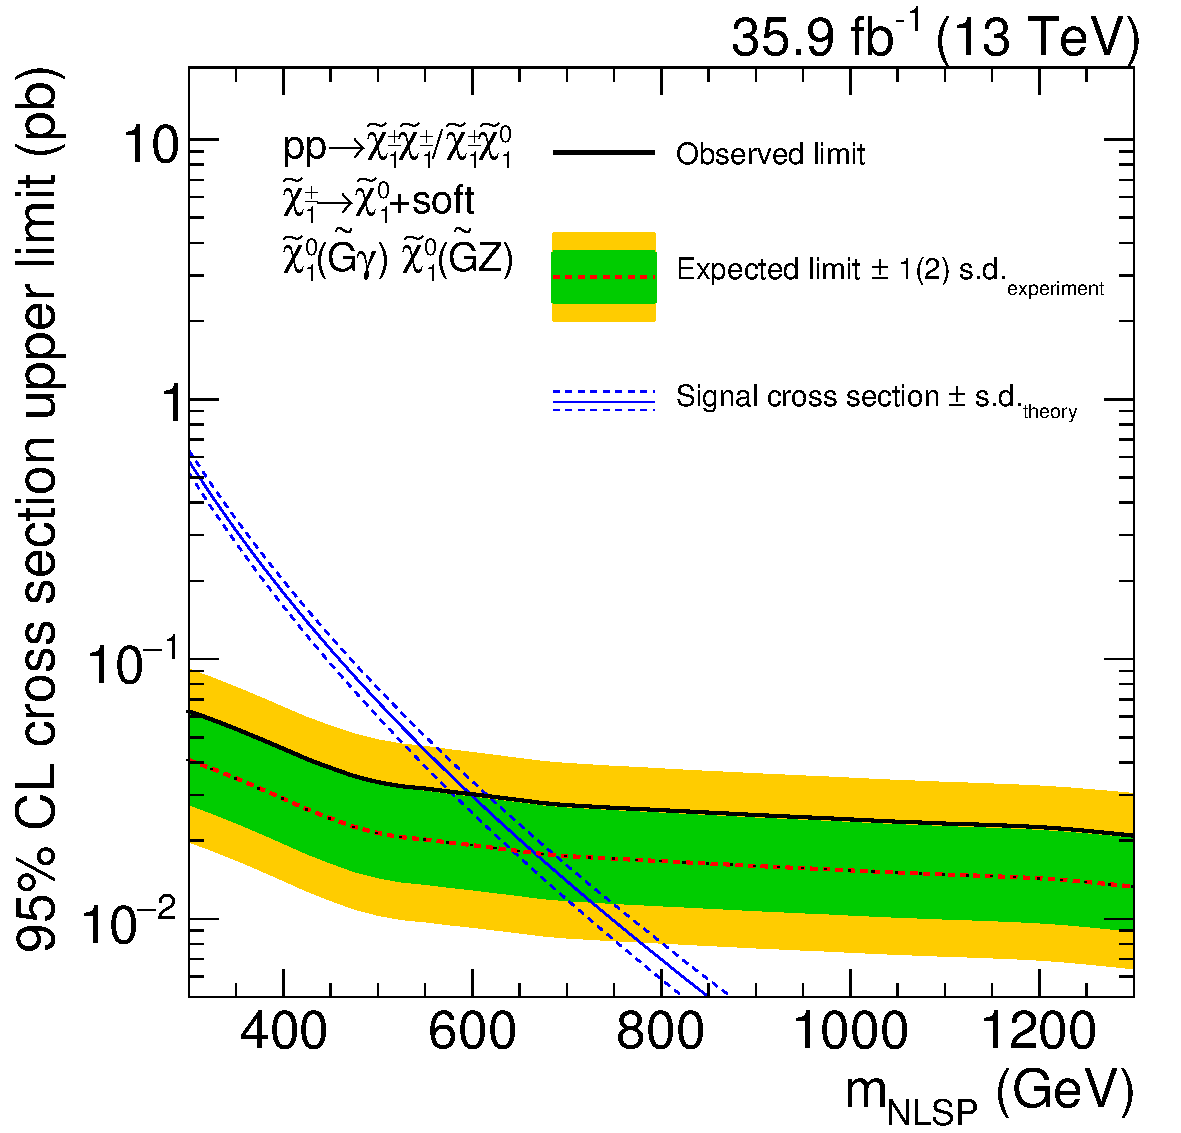
\includegraphics[width=0.55\textwidth]{figures/EndorsementPlots/TChiNG_limit2}\\
 \vspace{\baselineskip}
 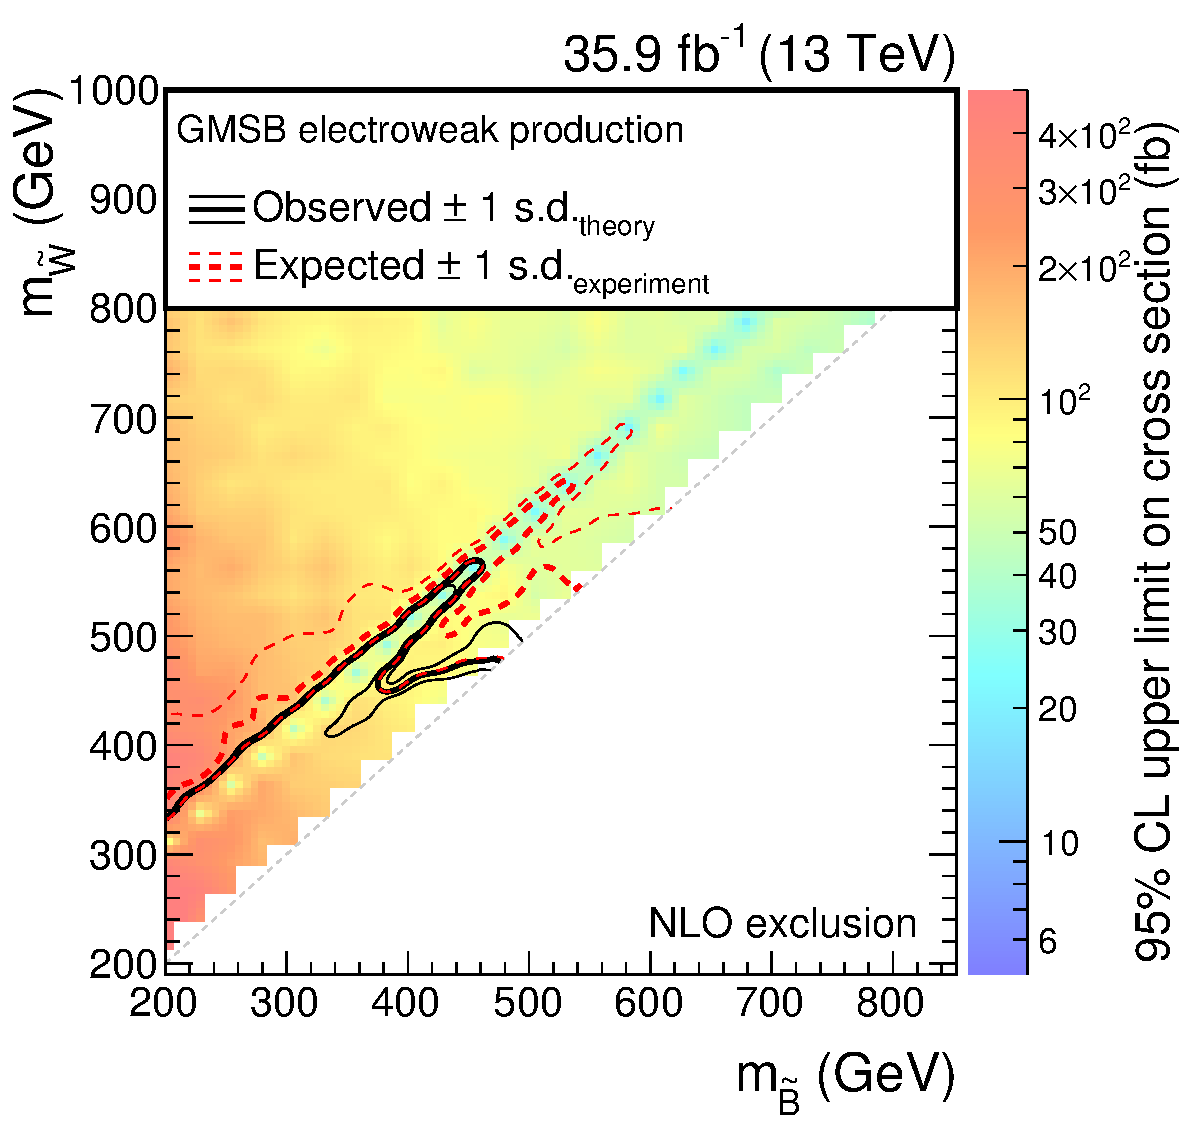
\includegraphics[width=0.65\textwidth]{figures/EndorsementPlots/GMSB_limits_XSEC2}
 \caption{Expected and observed upper limits for the \texttt{TChiZG} electroweak SMS (top) and the full GMSB model (bottom).}
 \label{fig:limitEWK}
\end{figure}

% \begin{figure}[btp]
%  \centering
%.481 = pairwidth
% 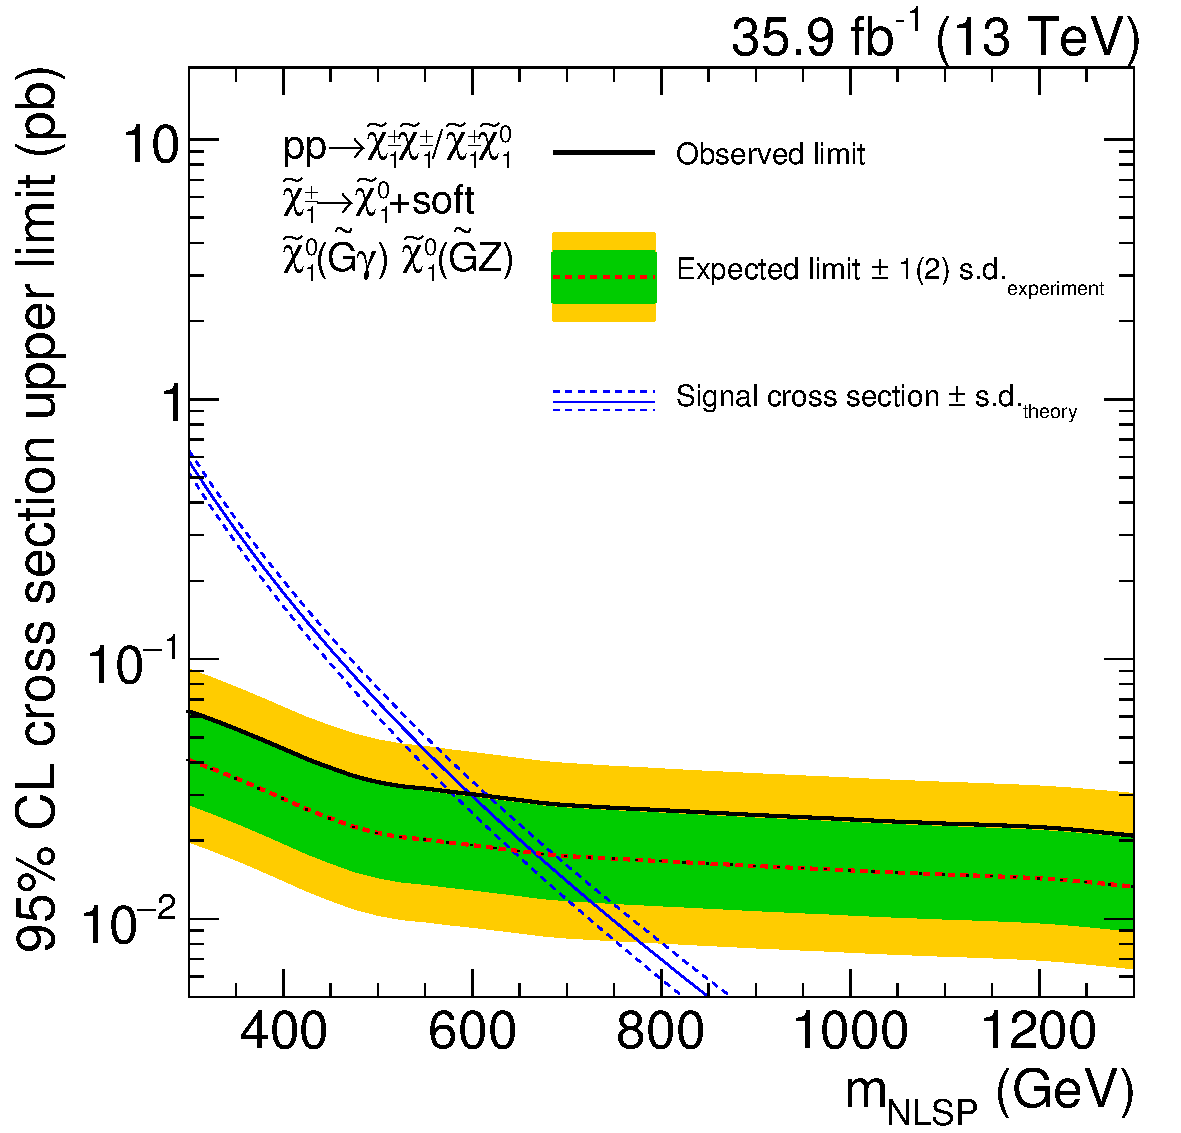
\includegraphics[width=0.449\textwidth]{figures/EndorsementPlots/TChiNG_limit2}
%  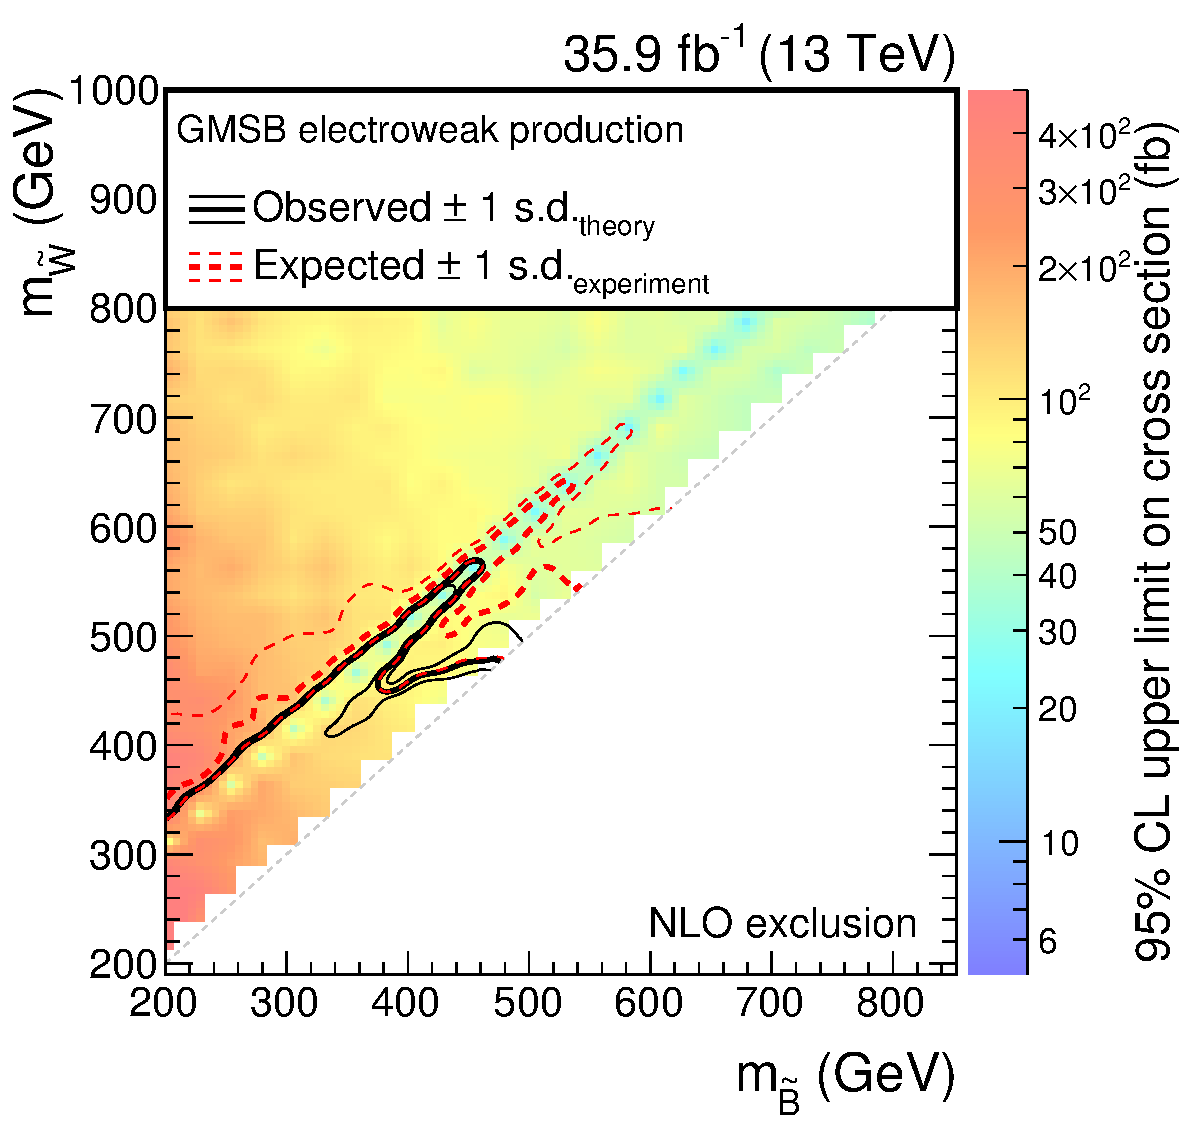
\includegraphics[width=0.6\textwidth]{figures/EndorsementPlots/GMSB_limits_XSEC2}
%  \caption{Expected and observed upper limits for the \texttt{TChiZG} electroweak SMS (left) and the full GMSB model (right).}
%  \label{fig:limitEWK2}
% \end{figure}
\newpage
\subsubsection*{Limits on strong production of gluinos}
In addition to the limits on EWK SUSY production, the results are interpreted in an SMS with gluino pair production. The cross section upper limits are shown in \refFig{fig:limitStrong} in the gluino-NLSP mass plane.\\
The analysis can exclude gluino masses up to $1.4\TeV$, depending on the mass of the NLSP, and thus the mass splitting between them. For NLSP masses lower than $150\GeV$, the sensitivity drops because of the applied $\mtTwo$ threshold of $100\GeV$. Because $\mtTwo$ yields an estimate of the NLSP mass, but the $\mtTwo$ distribution shows an endpoint at the NLSP mass and is broad due to the difficulty in the interpretation of $\ptmiss$ in the calculation, signal points with NLSP masses above $100\GeV$ are also affected by this requirement. With increased $\neutralinoOne$ masses the sensitivity rises, since the final state products carry more energy. Again, the same effect between expected and observed limit contour is observable as for the electroweak models.\\
In addition, comparing the cross section limits over the parameter space, statistical fluctuations are present because of the limited number of events being simulated in the SMS. This reflects also the large fluctuation which was observed in the variation range of the statistical and systematic uncertainties. Moreover, the small differences in the cross section limit indicate that the sensitivity is almost similar for varying NLSP masses, and the exclusion contour is mainly determined by the production cross section and the small branching fraction of the $\PZ$ boson to leptons.

\begin{figure}[tbp]
 \centering
 % 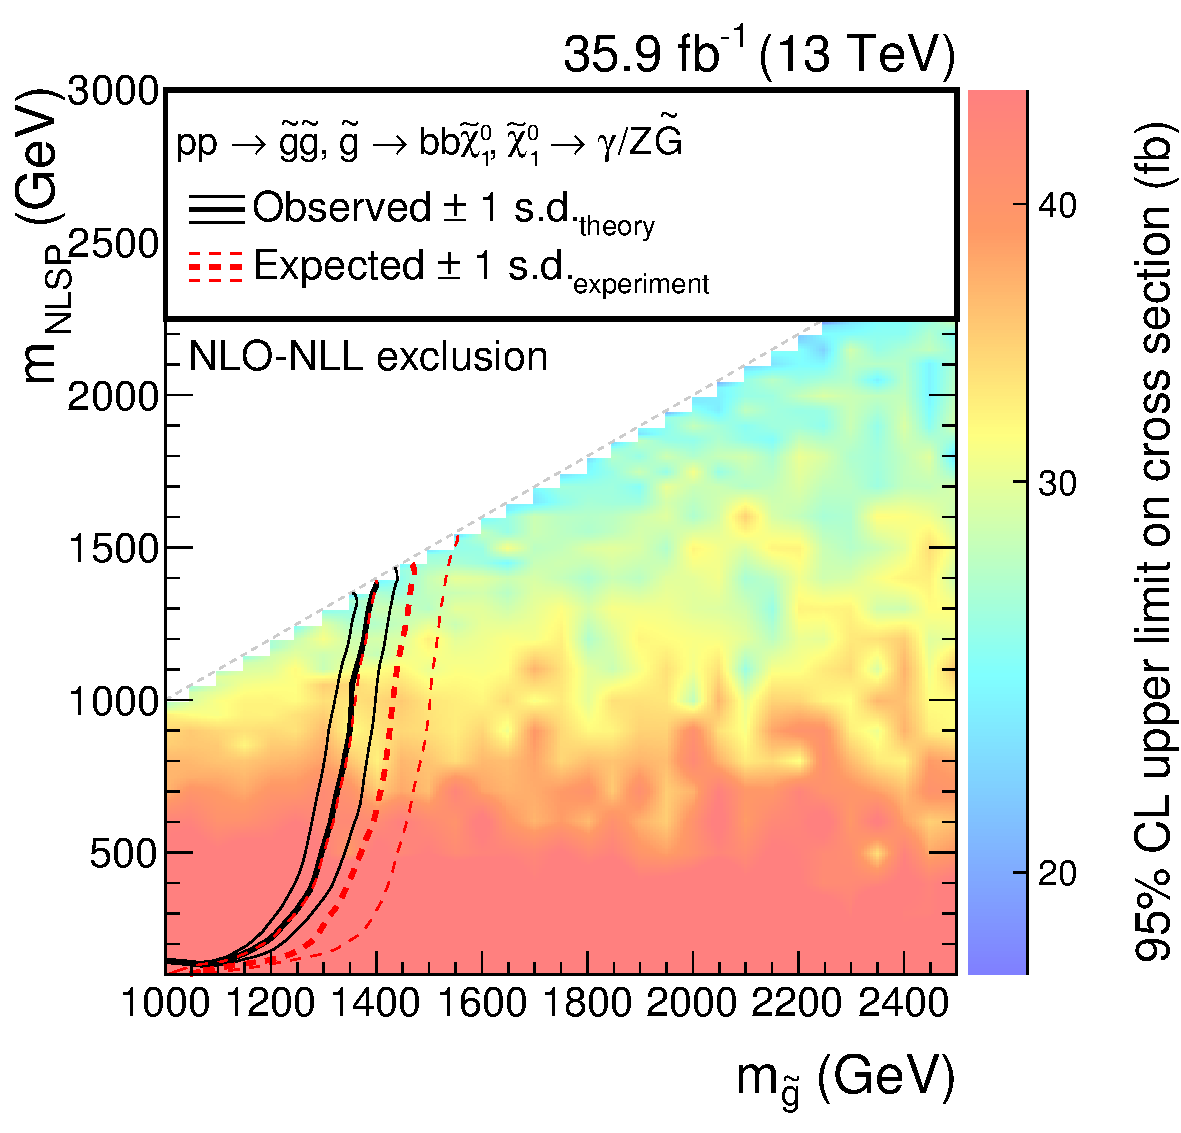
\includegraphics[width=\pairwidth]{figures/EndorsementPlots/T5bbbbZg_limits_XSEC2}
 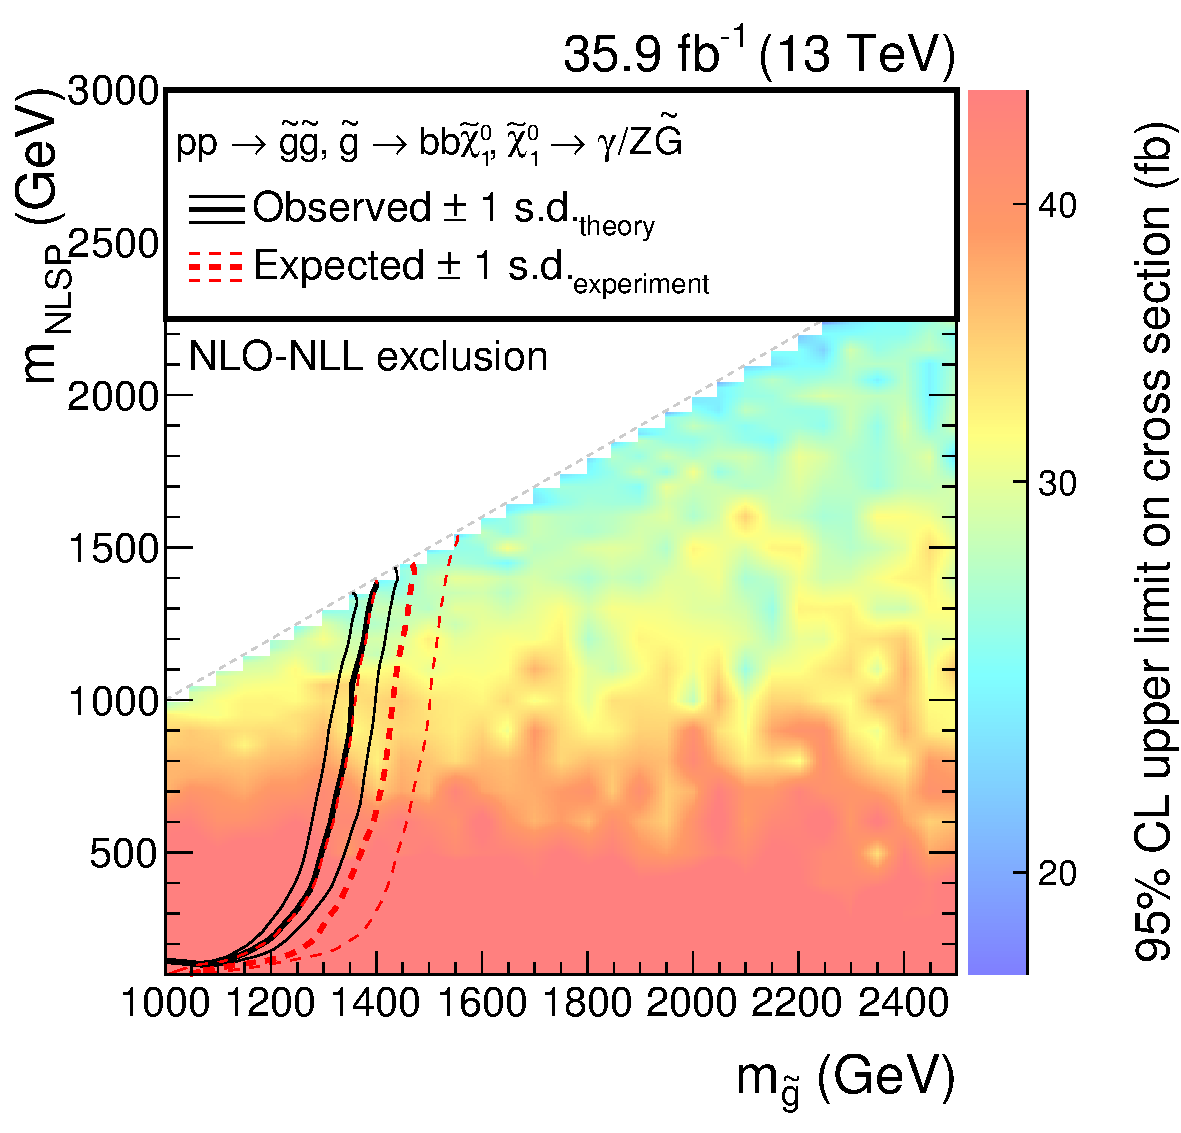
\includegraphics[width=0.65\textwidth]{figures/EndorsementPlots/T5bbbbZg_limits_XSEC2}
 \caption{Expected and observed upper limits for the \texttt{T5bbbbZG} SMS with strong production.}
 \label{fig:limitStrong}
\end{figure}
